\newcounter{nc}
\section{Introduction}
A notional example with two supply bases and two demand bases is utilized for analysis. The model is initially solved given a specific expected demand for each priority type. With two priority types, Priority 1 or ``Super/999/1" and Priority 2/3, and quantiles of real world expected demand, there are 25 expected demand combinations for which the model is run. Stochasticity in demand is analyzed post-solution to ascertain if categorical assumptions on demand affect aircraft allocation and to assess the monetary penalties associated with shorting or exceeding demand in the event of mis-estimation.

\section{Pre-Analysis Processing}
Considered for analysis are the transports from the continental United States (CONUS) to anywhere else in the world (OCONUS). Channels with highest total shipping volume deriving from each of the East and West coasts of CONUS are McGuire AFB (KWRI) to Ramstein AB (ETAR) and Travis AFB (KSUU) to Osan AB (RKSO). Due to the high volume of shipments over these channels, analyses of the expected demand is on the weekly demand. A combined list of demand over the 2017 and 2018 fiscal years (FY) for KWRI to ETAR and KSUU to RKSO results in 44 data points per priority type. There are four less data points per priority type than expected because shipments between McGuire AFB and Ramstein AB were not reported in FY 2018 April-July. The quantiles for the respective demand of each priorities can be seen in Table \ref{table_quantiles}.
\begin{table}[H]
    \centering
    \caption{Quantiles for Expected Demand}
    \begin{tabular}{@{}ccc@{}}
    \toprule
    Percentile & Super/999/1 & Priority 2/3 \\ \midrule   
    0th & 22  & 13   \\
    25th & 50  & 21\\
    50th & 80  & 30 \\
    75th & 106 &35\\
    100th & 155 &49\\ \bottomrule
    \end{tabular}
    \label{table_quantiles}
\end{table}


Aircraft availability is determined by the number of each aircraft type necessary to carry the maximum cargo quantiles to each selected OCONUS location. In this instance, there is a maximum total demand across OCONUS bases of 310 pallets of Super/999/1 cargo and 98 pallets of Priority 2/3 cargo or a total of 408 pallets and 1060.8 Klbs. Between space capacity and weight capacity, the limiting factor for number of aircraft is space capacity.  For the notional example, available aircraft are set as the number of aircraft to ship the maximum average demand level for both priority types for one week. The aircraft requirements of each MDS for the maximum demand level are 12 C-5s, 23 C-17s, or 51 C-130s. The GAMS model is ran 25 times, each instance solving for a different expected demand quantile combination. After each run, aircraft and cargo allocations are saved in an Excel file and a final cost for the demand combination is computed. The final result is a set of 25 point estimates for cost given differing expected demand amounts for two cargo types.   

\section{Actualizing Demand} \label{section_analysis_postprocessing}
After model processing an initial cost frontier is created. Figure \ref{fig_noPriorityCost} shows that there is not a correlation between number of pallets shipped and cost per pallet.
\begin{figure}[H]
\centering
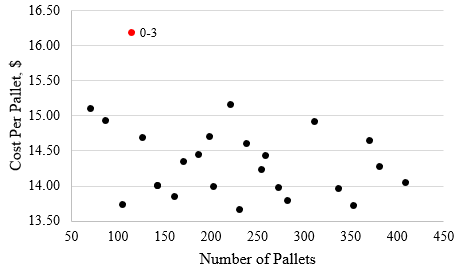
\includegraphics[width=110mm]{analysis_noPriorityCost_03.PNG}
\caption{Graph Cost per Pallet vs. Number Pallets: No Priority Cost}
\label{fig_noPriorityCost}
\end{figure}
Of note, the quantile combination of the minimum for Super/999 cargo and the 75th percentile for Priority 2/3 cargo results in the highest cost per pallet over all other demand pairings. The only visible reason for this disparity in cost is that out of the 10 aircraft allocated to ship 57 pallets to each base, two C-5s from KWRI to ETAR and 8 C-130s from KSUU to RKSO, one C-5 utilizes only 58.3\% of the pallet slots and one C-130 utilizes a mere 12.5\%. \par 
To assess stochasticity in demand, a cost frontier for the 25 cost estimates is created that accounts for an ``actual" demand that is realized post solution processing. Graphing the demand data suggests that the Super/999/1 cargo may be modeled by a uniform distribution, while the Priority 2/3 cargo follows a triangular distribution.

\begin{figure}[H]
\centering
\begin{minipage}[b]{0.4\textwidth}
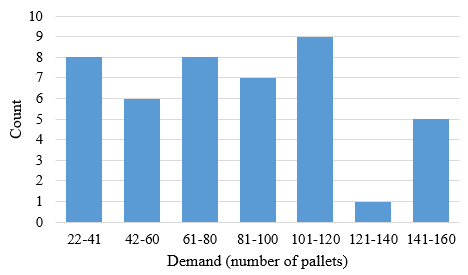
\includegraphics[width=65mm]{analysis_histogramSuper.PNG}
\caption{Histogram of Super/999/1 Cargo}
\label{fig_histogramSuper}
\end{minipage}
\hspace{10mm}
\begin{minipage}[b]{0.4\textwidth}
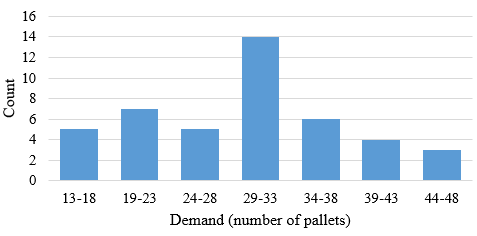
\includegraphics[width=65mm]{analysis_histogramStd.PNG}
\caption{Histogram of Priority 2/3 Cargo}
\label{fig_histogramStd}
\end{minipage}
\end{figure}
Demand distributions are created using data parameters for each of the cargo types, found in Table \ref{table_triangular}. One hundred demand samples are populated through random draws from the corresponding distributions.
\begin{table}[H]
\centering
\caption{Data Parameters per Priority Type}
\label{table_triangular}
\begin{tabular}{@{}lcc@{}}
\toprule
 & Super/999/1 & Priority 2/3 \\ \midrule
Min & 22 & 13 \\
Mode & N/A & 32 \\
Max & 155 & 49 \\ \bottomrule
\end{tabular}
\end{table}
The amount of excess and shortage of cargo of each type is calculated and multiplied by a priority cost depending on type of offense (excess or shortage) and cargo type. Several priority cost schema are used since ``real world" cost consequences are not documented for the generic cargo descriptions of Super/999/1 or Priority 2/3.  

\section{Fixed Cost Models}
Initial penalty cost models set a fix cost for shorting or exceeding the actual demand for each cargo priority type.  The first penalty cost allotment is arranged so that all penalty costs are the same. Tables \ref{table_penaltyCost1111} and \ref{table_top3_1111} depict the costs and demand combinations, respectively, for Model\refstepcounter{nc}\label{FC_1111} \ref{FC_1111}. As Table \ref{table_top3_1111} shows, the least costly demand combination given the penalty costs are all the same and at the equivalent of one kilo-pound of jet fuel, is setting the expected demand for Super/999 to the 50th percentile and Priority 2/3 to the 75th percentile.
\begin{table}[H]
\centering
\begin{minipage}[b]{0.4\textwidth}
\caption{Penalty Cost Model \ref{FC_1111}}
\label{table_penaltyCost1111}
\begin{tabular}{@{}lcc@{}}
\toprule
 & Super/999/1 & Priority 2/3 \\ \midrule
Excess & 1 & 1 \\
Short & 1 & 1 \\ \bottomrule
\end{tabular}
\end{minipage}
\hspace{10mm}
\begin{minipage}[b]{0.4\textwidth}
\caption{Top Demand Combinations for Penalty Cost Model \ref{FC_1111}: Quantile/Demand Amount}
\label{table_top3_1111}
\begin{tabular}{@{}lcc@{}}
\toprule
 & Super/999/1 & Priority 2/3 \\ \midrule
1 & 50\% / 80 & 75\% / 35 \\
2 & 25\% / 50 & 50\% / 30 \\
3 & 75\% / 106 & 75\% / 35 \\ \bottomrule
\end{tabular}
\end{minipage}
\end{table}


The second penalty cost model is arranged so that shorting Super/999/1 cargo is two times more offensive than shorting Priority 2/3 cargo and four times more offensive than exceeding Priority 2/3 cargo. With this cost model, depicted in Table \ref{table_penaltyCost1}, the three expected demand combinations with the lowest cost per pallet can be seen in Table \ref{table_top3_1}. These three combinations remain the top contenders even when the penalty costs of Model\refstepcounter{nc}\label{FC_4321} \ref{FC_4321} are all doubled.   

\begin{table}[H]
\centering
\begin{minipage}[b]{0.4\textwidth}
\caption{Penalty Cost Model \ref{FC_4321}}
\label{table_penaltyCost1}
\begin{tabular}{@{}lcc@{}}
\toprule
 & Super/999/1 & Priority 2/3 \\ \midrule
Excess & 3 & 1 \\
Short & 4 & 2 \\ \bottomrule
\end{tabular}
\end{minipage}
\hspace{10mm}
\begin{minipage}[b]{0.4\textwidth}
\caption{Top Demand Combinations for Penalty Cost Model \ref{FC_4321}: Quantile/Demand Amount}
\label{table_top3_1}
\begin{tabular}{@{}lcc@{}}
\toprule
 & Super/999/1 & Priority 2/3 \\ \midrule
1 & 50\% / 80 & 75\% / 35 \\
2 & 75\% / 106 & 75\% / 35 \\
3 & 75\% / 106 & 50\% / 30 \\ \bottomrule
\end{tabular}
\end{minipage}
\end{table}
The result of Model \ref{FC_4321} makes sense, because expecting demand to be at the 50th percentile or higher ensures that the egregious error of shorting an order is mitigated for both cargo types. This is especially true for Priority 2/3 cargo since the mode of the given data is 32, therefore expecting a demand of 35 will avoid shorting a shipment compared to assuming a demand of 30. \par
The third cost model, seen in Table \ref{table_penaltyCostTover}, places emphasis on not exceeding actual demand. The penalty cost for sending too much of a product doubles sending too little. Two of the three combinations with the least cost for Model\refstepcounter{nc}\label{FC_Tover} \ref{FC_Tover}, Tables \ref{table_penaltyCostTover} and \ref{table_top3_Tover}, differ from Model \ref{FC_4321}. The second contender in Model \ref{FC_Tover}, setting Super/999/1 cargo at the 50th percentile and Priority 2/3 at the 75th percentile, is Model \ref{FC_1111} and \ref{FC_4321}'s most economical expected demand combination. 
\begin{table}[H]
\centering
\begin{minipage}[b]{0.4\textwidth}
\caption{Penalty Cost Model \ref{FC_Tover}}
\label{table_penaltyCostTover}
\begin{tabular}{@{}lcc@{}}
\toprule
 & Super/999/1 & Priority 2/3 \\ \midrule
Excess & 2 & 2 \\
Short & 1 & 1 \\ \bottomrule
\end{tabular}
\end{minipage}
\hspace{10mm}
\begin{minipage}[b]{0.4\textwidth}
\caption{Top Demand Combinations for Penalty Cost Model \ref{FC_Tover}: Quantile/Demand Amount}
\label{table_top3_Tover}
\begin{tabular}{@{}lcc@{}}
\toprule
 & Super/999/1 & Priority 2/3 \\ \midrule
1 & 25\% / 21 & 50\% / 30 \\
2 & 50\% / 80 & 75\% / 35 \\
3 & 25\% / 21 & 25\% / 21 \\ \bottomrule
\end{tabular}
\end{minipage}
\end{table}
The fourth penalty cost model\refstepcounter{nc}\label{FC_Tshort}, Table \ref{table_penaltyCostTshort}, is the opposite of Model \ref{FC_Tover}'s; shorting demand is twice as egregious as exceeding. The same expected demand combinations for the first two are not only the same as Model \ref{FC_4321}, but also remain the same even when the fixed costs are doubled and quadrupled.
\begin{table}[H]
\centering
\begin{minipage}[b]{0.4\textwidth}
\caption{Penalty Cost Model \ref{FC_Tshort}}
\label{table_penaltyCostTshort}
\begin{tabular}{@{}lcc@{}}
\toprule
 & Super/999/1 & Priority 2/3 \\ \midrule
Excess & 1 & 1 \\
Short & 2 & 2 \\ \bottomrule
\end{tabular}
\end{minipage}
\hspace{10mm}
\begin{minipage}[b]{0.4\textwidth}
\caption{Top Demand Combinations for Penalty Cost Model \ref{FC_Tshort}: Quantile/Demand Amount}
\label{table_top3_Tshort}
\begin{tabular}{@{}lcc@{}}
\toprule
 & Super/999/1 & Priority 2/3 \\ \midrule
1 & 50\% / 80 & 75\% / 35 \\
2 & 75\% / 106 & 75\% / 35 \\
3 & 100\% / 155 & 25\% / 21 \\ \bottomrule
\end{tabular}
\end{minipage}
\end{table}
 Presuming the assumption of distributions for the cargo types is correct, setting expected demand to the 50th percentile for Super/999/1 cargo and to the 75th percentile for Priority 2/3 cargo is a preference in the fixed cost models. 
\section{Variable Cost Models}
The original pallet cost is the fuel amount required to fly aircraft with a specified cargo amount from a source to a destination and return to the source empty. Taking into consideration that under-shipping or over-shipping an item may require back-filling an order or returning the overage amount, respectively, the penalty cost can be viewed as a percentage of the cost to transport the pallet. The penalty cost could be the full pallet cost to account for a back-order or a range of percentages to account for the return of the pallet. The portion of flight costs associated with transporting cargo ranges from approximately 50 to 57 percent.\par
Setting the penalty cost amount to 100 percent for all cargo grievances for Model\refstepcounter{nc}\label{PC_100} \ref{PC_100} results in the least costly demand combinations for pallet costs, as seen in Table \ref{table_top3_PC100}, differing from their original penalty-free costs by only approximately four percent and the most costly by almost 160 percent. Figure \ref{fig_GraphNoPriorityCost} shows the effect of penalty costs on the cost per pallet when all penalty costs are equal to the original cost per pallet.  
\begin{table}[H]
    \centering
    \caption{Top Demand Combinations for Penalty Cost Model \ref{PC_100}: Quantile/Demand Amount}
    \label{table_top3_PC100}
    \begin{tabular}{@{}lcc@{}}
    \toprule
        & Super/999/1 & Priority 2/3 \\ \midrule
        1 & 25\% / 50 & 50\% / 30 \\
        2 & 25\% / 50 & 25\% / 21 \\
        3 & 25\% / 50 & 75\% / 35 \\ \bottomrule
    \end{tabular}
\end{table}

\begin{figure}[H]
\centering
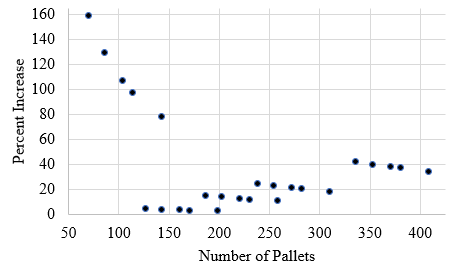
\includegraphics[width=105mm]{analysis_percent_100.PNG}
\caption{Graph Percentage Increase of Cost per Pallet vs. Number Pallets: Cost Model \ref{PC_100} (100\% Penalty)}
\label{fig_GraphNoPriorityCost}
\end{figure}

Keeping the shortage penalty constant at 100\% of the pallet cost, the final cost per pallet of the top (least costly) three demand combinations for the different proportional overage penalties are shown in Figure \ref{fig_GraphAllPercent}. Final cost per pallet does not strictly increase with an increase of penalty cost due to a shift in expected demand. Figure \ref{fig_Graph_PercentQuantiles} depicts the demand percentile of the foremost least costly demand combination over the different variable overage penalty costs. From this figure, there is a distinct expected demand quantile for each cargo type that results in the lowest total cost per pallet with a stochastic realized demand. In this instance, the expected demand quantity for a majority of the range of costs are the 75th percentile for Super/999/1 cargo and the 50th percentile for Priority 2/3 cargo.     

\begin{figure}[H]
\centering
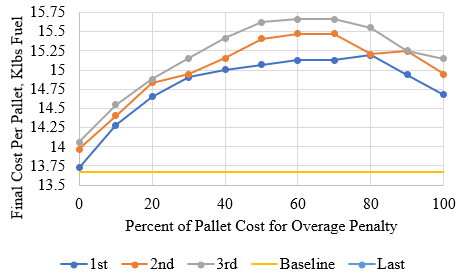
\includegraphics[width=105mm]{analysis_percent_All_Top3.PNG}
\caption{Graph Cost per Pallet vs Percentage of Pallet Cost for Overage Penalty}
\label{fig_GraphAllPercent}
\end{figure}

\begin{figure}[H]
\centering
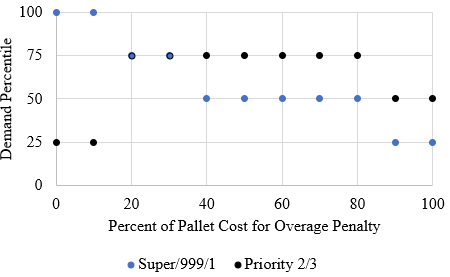
\includegraphics[width=105mm]{analysis_percent_Quantiles.PNG}
\caption{Graph Top Demand Percentile vs Percent of Pallet Cost for Overage Penalty}
\label{fig_Graph_PercentQuantiles}
\end{figure}

\section{Aircraft Allocation}
One finding with the notional example is that no C-17s were allocated to transport cargo from CONUS to the chosen OCONUS bases of Ramstein AB and Osan AB. This is likely due to the similar fuel efficiency between the C-5 and C-17 and that the C-5 has a higher cargo throughput compared to the C-17 when not accounting for mission capable rates \cite{Reiman2014}. Figure \ref{fig_numAircraft} depicts the number of aircraft allocated to fly for a given number of pallets.  Due to the lighter pallet weight of 2.6 Klbs, the C-130 is more fuel efficient compared to the C-17 and C-5.
%stupid column chart would not work, couldn't alter the ridiculous horizontal axis bounds because it thought it was categorical. Made scatter plot instead and added lines because it makes it easier to see where things are vs No-lines, but dimmed the lines to it's possibly more clear that the points are more important to note??? 
\begin{figure}[H]
\centering
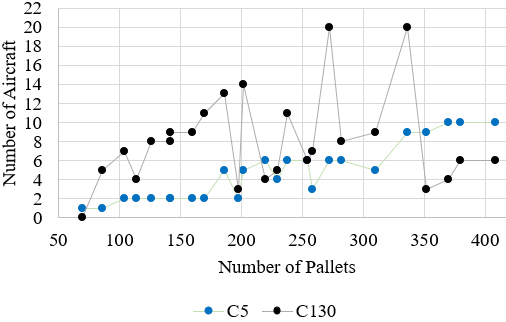
\includegraphics[width=105mm]{analysis_numC5andC130.PNG}
\caption{Graph Number of Aircraft vs Number of Pallets}
\label{fig_numAircraft}
\end{figure}

\textcolor{red}{Add figure of Costs vs Num Pallets with solely using each MDS}
